% !TEX root = ../main.tex
\section{Method} % (fold)
\label{sec:method}

After having reviewed recent research on fingerprinting, we turn to test the technique. Unfortunately due to the limited scope of this seminar paper we will focus on a small scale example fingerprinting of the aforementioned \texttt{HTTP-Header} values. 

\subsection{User recognition}
\label{subsec:userrecognition}
To test the described fingerprinting method, we create a small online fingerprinting service. In a live scenario, we will depend on recognizing revisiting users to leverage this service properly. When seeing User $U$, represented by his browser, having $n$ fingerprints $f_1, f_2, \ldots, f_n$ in our database, several things can occur:

\begin{itemize}
	\item $(1)$ (\emph{True Positive}): $U$ has visited already and we \textit{correctly} connect him to Fingerprint $f_U$.
	\item $(2)$ (\emph{False Positive}): $U$ has not visited yet and we \textit{falsely} connect him to Fingerprint $f_V$ or create a new one.
	\item $(3)$ (\emph{False Negative}): $U$ has visited already but we \textit{falsely} do not connect her with the correct $f_U$, instead creating a new one.
	\item $(4)$ (\emph{True Negative}): $U$ has not visited yet and we \textit{correctly} connect her to a new Fingerprint $f_U$.
	\label{item:cases}
\end{itemize}

\begin{wrapfigure}{r}{0.5\textwidth}
\centering
\frame{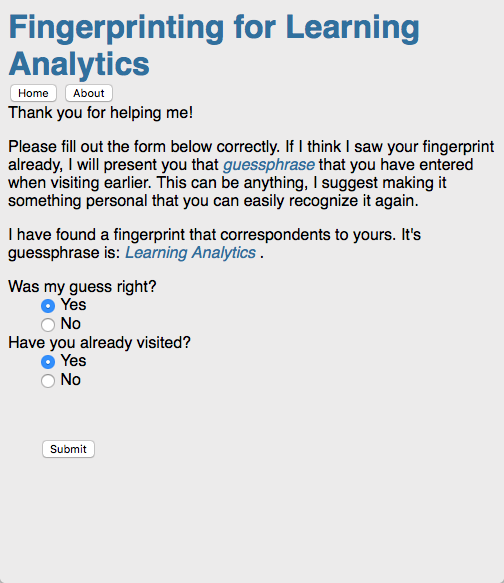
\includegraphics[height=3in]{img/fphp_secondvisit.png}}
\caption{Screenshot from \texttt{laprint}}
\label{fig:fpscreen}
\end{wrapfigure}
In order to get a rough estimate, how well we are able to hit cases $1$ and $4$ we will need some way to tell if we recognized users correctly. In a real life scenario this might be hard, but in our test case we can use an identifying phrase which we will call a \emph{guessphrase}. New users will be asked to provide such a identifying \emph{guessphrase} (e.g. name of first cat) which we will save together with the fingerprint. Revisiting users will be presented their \emph{guessphrase} and should tell, which of the above cases apply to them. This will of course be limited to a device and browser combination, since we are aiming for \emph{browser fingerprints} as explained in section \ref{sec:sota}. 

\subsection{Fingerprint creation}
\label{subsec:fingerprintvals}

We will limit our fingerprint to the basic \texttt{HTML} focused features. These should provide enough information to differentiate the small set of users. This will also facilitate the analysis, because we will only need to compare strings of features. Comparing different renderings in \texttt{WebGL} would introduce significant overhead in the sample implementation, whilst the main goal is to test recall and precision of the technique.

In Figure \ref{met:fig:headers} you can find all \texttt{HTTP-header} attributes we have collected from visiting users, together with values from one example visitor.


This recognition test, to again emphasize, aims to create a \textit{browser fingerprint}, not a \textit{device fingerprint}. In order to form the latter, additional feature extracted from the underlying hardware would be needed, which goes beyond the extent of this work. Cao and colleagues have already pointed out possibilities for doing so \cite{cao_cross-browser_2017}.

To test recall and precision for the fingerprints described in subsection \ref{subsec:userrecognition},we created a web service called \emph{Fingerprinting for Learning Analytics} which we used to fingerprint incoming users.\footnote{Inspired by the work of \href{amiunique.org}{amiunique}, but more lightweight.} It works roughly as follows:
\begin{wrapfigure}{l}{0.5\textwidth}
\centering
\footnotesize
\begin{tabular}{|p{2cm}|p{3cm}|}
\hline
	\texttt{HTTP-header} attribute & example \\ \hline\hline
	\texttt{user-agent} & Mozilla/5.0 (Macintosh; Intel Mac OS X 10.11; rv:58.0) Gecko/20100101 Firefox/58.0\\\hline
	\texttt{accept\-language} & de,en-US;q=0.7,en;q=0.3 \\\hline
	\texttt{accept\-encoding} & gzip, deflate \\\hline
	\texttt{accept} & text/html, application/xhtml+xml, application/xml; q=0.9, */*; q=0.8 \\ \hline
\end{tabular}
\caption{Collected \texttt{HTTP-header} values.}
\label{met:fig:headers}
\vspace{-1in}
\end{wrapfigure}



\begin{itemize}
	\item (1) Ask an incoming user, if she/he agrees on saving fingerprinting features of her/his browser.
	\item (2) Create a fingerprint and associating it with the user's \emph{guessphrase}.
	\item (2a) In case the fingerprint was recognized, the \emph{guessphrase} was presented and the user was asked whether it's correct.
	\item (3) Save the result for later analysis.
\end{itemize}

This is implemented rather straightforward. If the user agrees, we collect the \texttt{HTTP-Header} Attributes seen in Figure \ref{met:fig:headers} from the \texttt{request} object that is being sent with every \texttt{HTTP}-request. The 4-tuple \texttt{$($User-Agent$,$ Accept$,$ Accept-Language$,$ Accept-Encoding$)$} constructs the fingerprint $f_U$. We query our database for $f_U$ to see if the User is known. If we have seen $f_U$ in connection with multiple \emph{guessphrases}, we chose one of them at random and present them to the user. We could also have thrown an error, but in a real life scenario we wouldn't want to interrupt the users experience. Another solution would have been to then fall back to a default user. 

\pagebreak
\subsection{xAPI integration}

\begin{wrapfigure}{l}{0.55\linewidth}
\centering
\tiny
\begin{verbatim}
{
  "id":"12345678",
  "actor":{
    "openid":"http://www.example.org/video1/fp?acceptEncoding=gzip
      ,deflate\&UserAgent=Mozilla/5.0(Macintosh;IntelMacOSX10.11;.."
  },
  "verb":{
    "id":"http://adlnet.gov/expapi/verbs/watched",
    "display":{
      "en-US":"watched"
    }
  },
  "object":{
    "id:":"http://example.adlnet.gov/xapi/example/activity"
  }
}
\end{verbatim}
\caption{Sample xAPI Statement with Fingerprint (modified from documentation)}
\label{fig:xapi}
\end{wrapfigure}

Another subject to touch on is the integration with other Educational Technology. To properly use fingerprinting for tracking educational experiences, we need to have these fingerprints conform to a standard. A standardized exchange format is \texttt{xAPI}\footnote{Specification available on GitHub: \href{https://github.com/adlnet/xAPI-Spec}{xAPI-Spec}.}. Since a fingerprint in general will refer to a user that visits a website, we will propose ways to construct an \texttt{actor} object, that can then be combined with other properties to form a statement. The triple of (\texttt{actor}, \texttt{verb}, \texttt{object}) is minimal. Note that it will be impossible to come up with a fully standard compliant way to implement a fingerprint as an \texttt{actor} object, since these are required to only identify one agent or a group of agents, which cannot be guaranteed by fingerprinting.

The first way to construct the \texttt{actor} object which would be most intuitive, is to simply store all fingerprint attributes. This would result in a user object that is similar to what the fingerprinting entity has seen, adding no further complication.
Unfortunately, the xAPI specification forbids an \texttt{actor} object to be customized and only allows it to have one out of four Inverse Functional Identifiers from which we can already exclude \texttt{mbox}, \texttt{mbox\_sha1sum} and \texttt{account}. If these could be obtain or created, fingerprinting would possibly be obsolete. 

The only way to construct a valid IFI would be to create an OpenID. The URI would begin with the site that the fingerprinted user has visited and then store all attributes in a form of query attributes.\footnote{e.g.: \texttt{http://www.example.org/video1/fp?acceptEncoding=gzip,deflate\&User Agent=Mozilla/5.0(Macintosh;IntelMacOSX10.11;}[...]} We would then have encapsulated the fingerprint in the \texttt{actor} object to build a statement with, as seen in Figure \ref{fig:xapi}.

% section introduction (end)